\documentclass[12pt,a4paper]{article}

% ============================================================
% PACKAGES
% ============================================================
\usepackage[
    a4paper,
    top=1.55cm,
    bottom=1.35cm,
    left=1.75cm,
    right=1.75cm
]{geometry}

\usepackage[T1]{fontenc}
\usepackage{newtxtext}
\usepackage{graphicx}
\usepackage{xcolor}
\usepackage{array}
\usepackage{tabularx}
\usepackage{fancyhdr}
\usepackage{tikz}
\usepackage{eso-pic}
\usepackage{ragged2e}

% ============================================================
% COLORS
% ============================================================
\definecolor{GEUBlue}{RGB}{43,91,145}
\definecolor{GEUBannerBlue}{RGB}{0,102,148}
\definecolor{GEUYellow}{RGB}{255,201,38}
\definecolor{InstructionGrey}{RGB}{125,125,125}

% ============================================================
% GENERAL SETTINGS
% ============================================================
\setlength{\parindent}{0pt}
\setlength{\parskip}{0pt}
\renewcommand{\arraystretch}{1.18}

% ============================================================
% HEADER / FOOTER
% ============================================================
\pagestyle{fancy}
\fancyhf{}

\fancyhead[L]{%
    \fontsize{10}{12}\selectfont
    CSE - DSCPP-III-2026-T226
}

\fancyhead[R]{%
    \fontsize{10}{12}\selectfont
    PHASE-II PROJECT PROGRESS
}

\fancyfoot[R]{%
    \fontsize{10}{12}\selectfont
    Page \thepage
}

\renewcommand{\headrulewidth}{0pt}
\renewcommand{\footrulewidth}{0pt}

\setlength{\headheight}{20pt}
\setlength{\headsep}{0.55cm}
\setlength{\footskip}{0.65cm}

% ============================================================
% BOTTOM YELLOW LINE
% ============================================================
\AddToShipoutPictureBG{%
\begin{tikzpicture}[remember picture,overlay]
    \fill[GEUYellow]
    (current page.south west)
    rectangle
    ([yshift=0.14cm]current page.south east);
\end{tikzpicture}
}

% ============================================================
% CUSTOM COMMANDS
% ============================================================
\newcommand{\sectiontitle}[1]{%
    {\color{GEUBlue}
    \fontsize{16.5}{20}\selectfont #1}
}

\newcommand{\instruction}[1]{%
    {\color{InstructionGrey}
    \fontsize{9.5}{12}\selectfont #1}
}

\newcommand{\answerbox}[2]{%
    \noindent
    \begin{tabularx}{\textwidth}{
        |>{\raggedright\arraybackslash}X|}
        \hline
        \parbox[t][#1][t]{\dimexpr\linewidth-12pt\relax}{
            \vspace{4pt}
            \fontsize{10}{13.5}\selectfont #2
        }\\
        \hline
    \end{tabularx}
}

% ============================================================
% DOCUMENT
% ============================================================
\begin{document}

% ============================================================
% PAGE 1
% ============================================================

\vspace*{0.05cm}


\includegraphics[width=7.5cm]{geulogo.png}

\vspace{0.45cm}

\noindent
\colorbox{GEUBannerBlue}{%
\parbox{\dimexpr\textwidth-2\fboxsep\relax}{
    \vspace{0.14cm}
    {\color{GEUYellow}
    \fontsize{15.5}{19}\selectfont
    \bfseries
    PROJECT AND TEAM INFORMATION}
    \vspace{0.14cm}
}}

\vspace{0.45cm}

% PROJECT TITLE
\sectiontitle{Project Title}

\vspace{0.03cm}

\instruction{}

\vspace{0.20cm}

\answerbox{1.05cm}{\textbf{Intelligent Traffic Optimization System}}

\vspace{0.45cm}

% STUDENT INFORMATION
\noindent
\begin{tabularx}{\textwidth}{|>{\RaggedRight\arraybackslash}p{0.46\textwidth}|>{\RaggedRight\arraybackslash}X|}
\hline
\begin{minipage}[t][1.10cm][c]{\linewidth}
\textit{Team Name:}\\[1pt]
\textit{Team \#}
\end{minipage}
&
\begin{minipage}[t][1.10cm][c]{\linewidth}
\textit{}\\
\textit{DSCPP-III-2026-T226}
\end{minipage}
\\
\hline
\begin{minipage}[t][2.95cm][t]{\linewidth}
\vspace{2mm}
\textbf{Team member 1 (Team Lead)}\\[1pt]
\textit{(Last Name, name: student ID: email, picture):}
\end{minipage}
&
\begin{minipage}[t][2.95cm][t]{\linewidth}
\vspace{2mm}
Akshita -- 2510012193\\
{\fontsize{9.5}{12}\selectfont\textit{akshitachourdhary8923@gmail.com}}

\vspace{2mm}
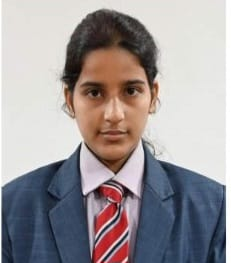
\includegraphics[width=2.8cm,height=1.45cm,keepaspectratio]{member1.png}
\end{minipage}
\\
\hline
\begin{minipage}[t][2.95cm][t]{\linewidth}
\vspace{2mm}
\textbf{Team member 2}\\[1pt]
\textit{(Last Name, name: student ID: email, picture):}
\end{minipage}
&
\begin{minipage}[t][2.95cm][t]{\linewidth}
\vspace{2mm}
Singh, Vaani -- 2510360148\\
{\fontsize{9.5}{12}\selectfont\textit{vaanisingh56@gmail.com}}

\vspace{2mm}
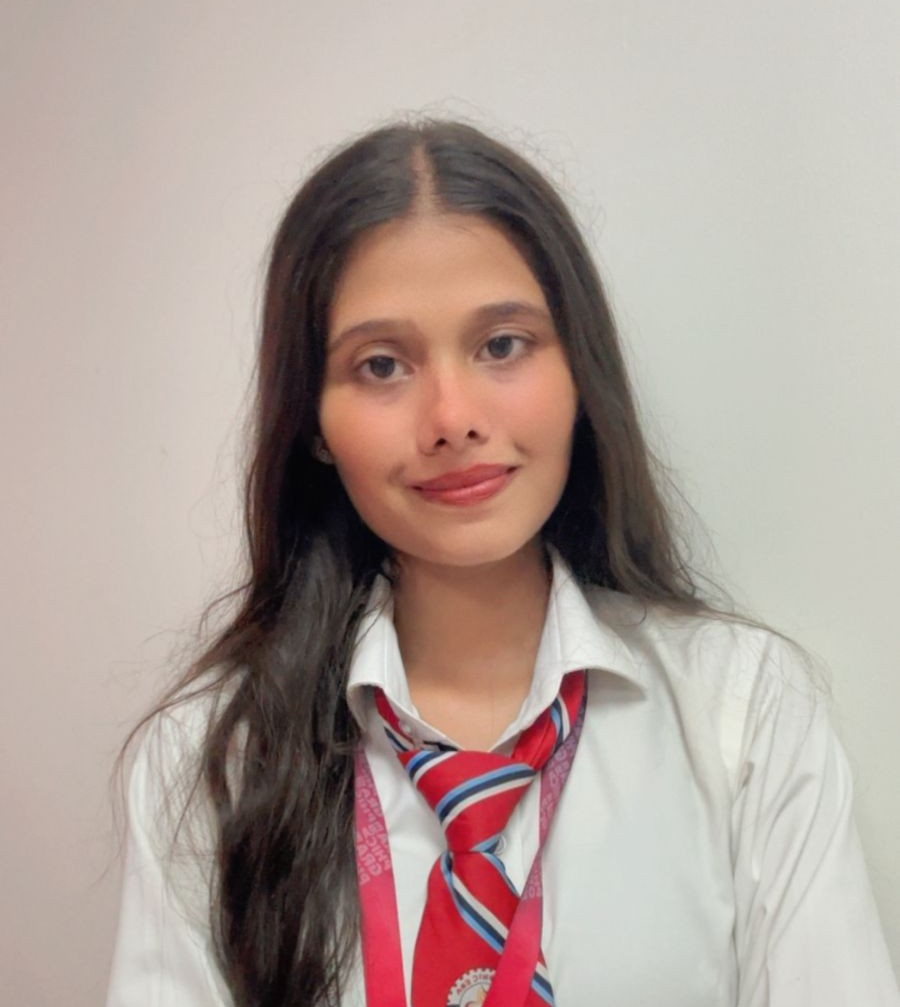
\includegraphics[width=2.8cm,height=1.45cm,keepaspectratio]{member2.png}
\end{minipage}
\\
\hline
\begin{minipage}[t][2.95cm][t]{\linewidth}
\vspace{2mm}
\textbf{Team member 3}\\[1pt]
\textit{(Last Name, name: student ID: email, picture):}
\end{minipage}
&
\begin{minipage}[t][2.95cm][t]{\linewidth}
\vspace{2mm}
Yadav, Panshu -- 2510350036\\
{\fontsize{9.5}{12}\selectfont\textit{Panshu.yadav22@gmail.com}}

\vspace{2mm}
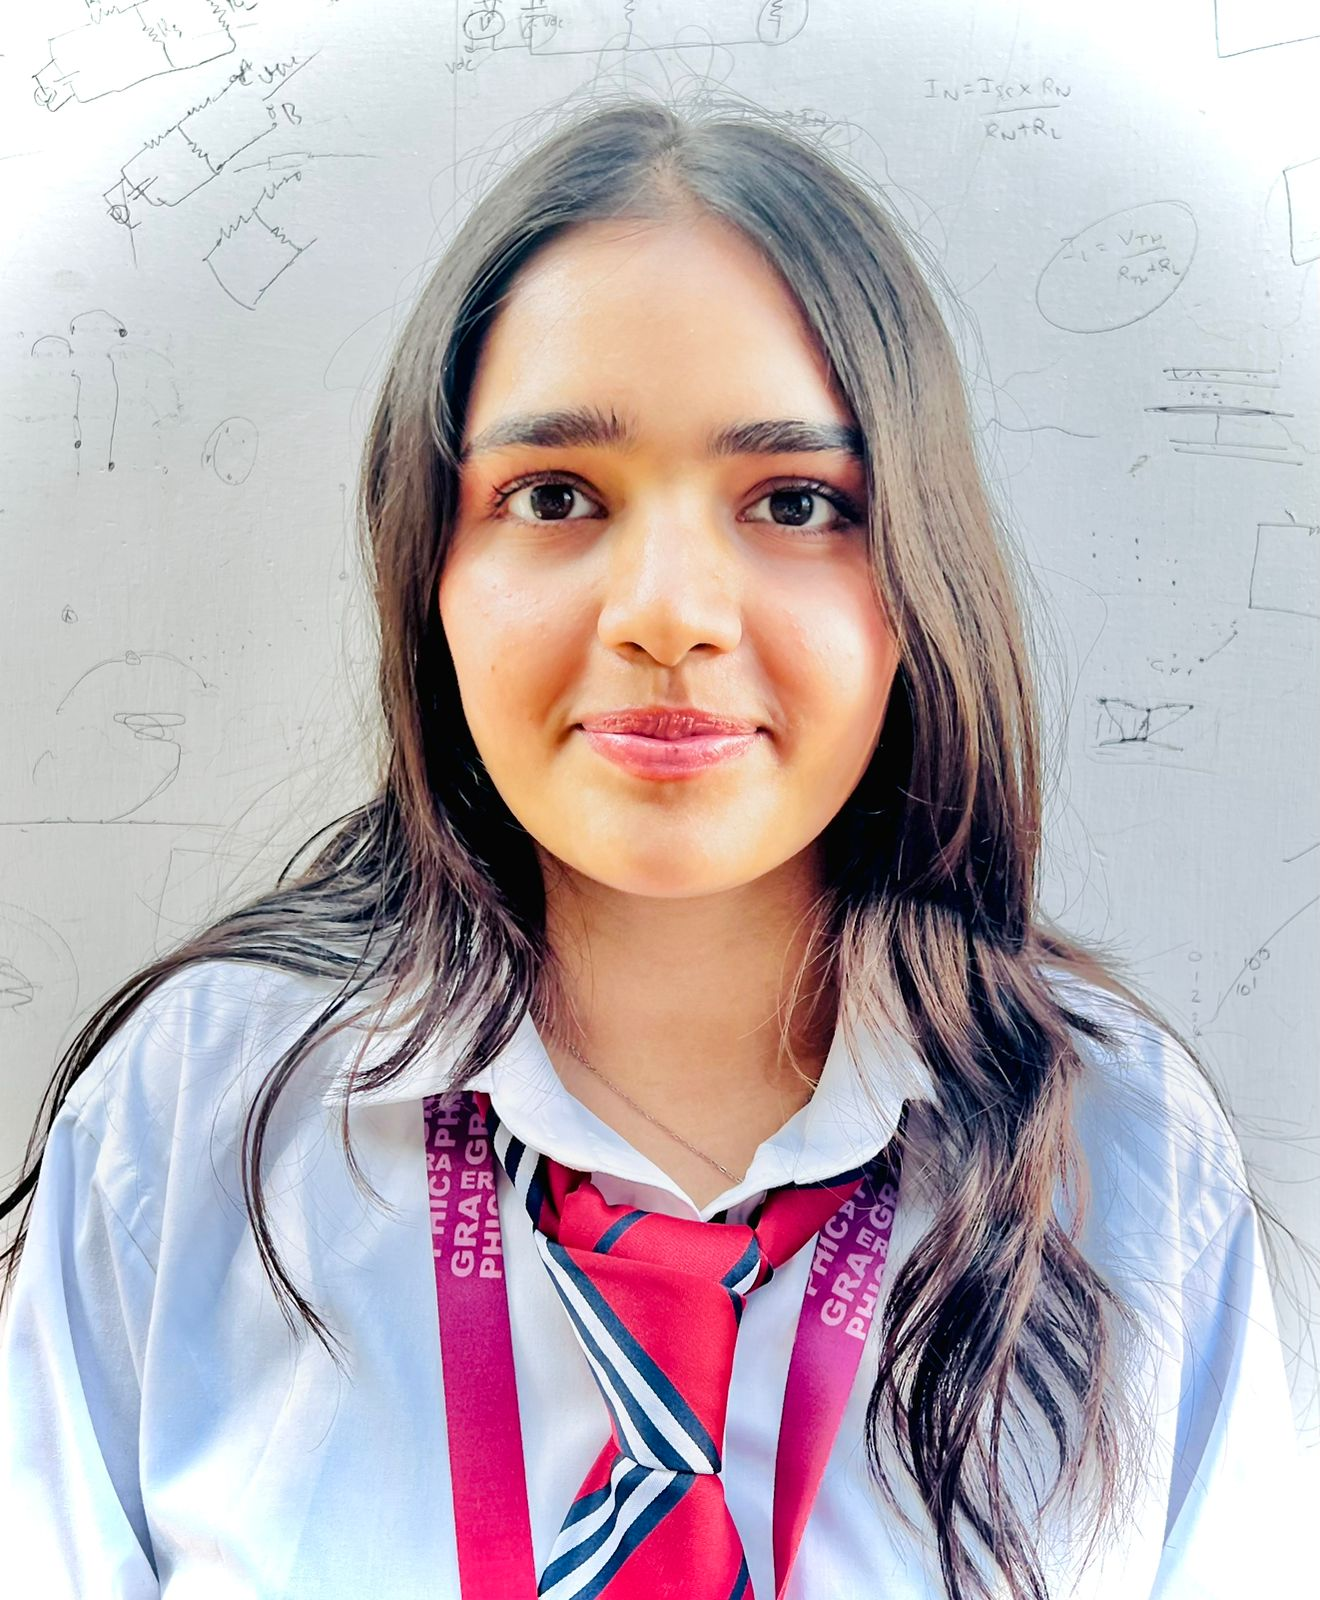
\includegraphics[width=2.8cm,height=1.45cm,keepaspectratio]{member3.png}
\end{minipage}
\\
\hline
\end{tabularx}

\newpage
% ============================================================
% PAGE 2
% ============================================================

\vspace*{0.05cm}

\noindent
\colorbox{GEUBannerBlue}{%
\parbox{\dimexpr\textwidth-2\fboxsep\relax}{
    \vspace{0.15cm}
    {\color{GEUYellow}
    \fontsize{15.5}{19}\selectfont
    \bfseries
    PHASE-II PROJECT PROGRESS DESCRIPTION (35 pts)}
    \vspace{0.15cm}
}}

\vspace{0.45cm}

% PROJECT ABSTRACT
\sectiontitle{Project Abstract}

\vspace{0.03cm}

\instruction{

}

\vspace{0.15cm}

\answerbox{4.60cm}{Urban traffic congestion stems from static, pre-programmed signal timers that fail to reflect dynamic vehicle distributions, causing unnecessary idle delays, elevated emissions, and fuel waste. Because physical road widening is often infeasible in dense city grids and complex roadside sensor infrastructure (such as inductive loop detectors or optical computer vision feeds) is cost-prohibitive for municipal deployment, an algorithmic approach is essential.

This project implements a high-efficiency discrete-event traffic simulation in modern C++. The system continuously tracks queue depths across intersection approaches, computes real-time traffic density, dynamically optimizes green-signal durations, and guarantees low-latency preemption for approaching emergency vehicles. By combining FIFO queues, max-heaps, adjacency graphs, and transition stacks, the platform optimizes overall vehicular throughput while enforcing starvation-prevention and safety constraints.}

\vspace{0.50cm}

% UPDATED PROJECT APPROACH
\sectiontitle{Updated Project Approach and Architecture}

\vspace{0.03cm}

\instruction{

}

\vspace{0.15cm}

\answerbox{8.20cm}{The system is architected in modern C++ applying object-oriented design patterns to simulate real-world intersection dynamics via dedicated data structures:
\begin{itemize}\setlength{\itemsep}{2.5pt}\setlength{\parskip}{0pt}\setlength{\leftskip}{-8pt}
    \item \textbf{FIFO Queues:} Model individual lane buffers, guaranteeing first-come, first-served vehicle traversal and realistic queuing behavior.
    \item \textbf{Priority Queue (Max-Heap):} Dynamically allocates green signal phases based on composite weights derived from approach queue depths, cumulative vehicle wait latencies, and high-priority emergency preemption flags.
    \item \textbf{Graph Structure (Adjacency List):} Represents the roadway network topology, with vertices denoting junctions and directed edges modeling multi-lane corridors.
    \item \textbf{Stack (LIFO):} Maintains an operational audit log of recent phase transitions to evaluate historical patterns, prevent rapid oscillation, and enforce fairness.
    \item \textbf{Doubly Linked List:} Manages active vehicle entities progressing through the intersection conflict zone with $O(1)$ insertions and removals.
\end{itemize}
\vspace{2pt}
The simulation pipeline operates through six modular engines: Vehicle Arrival Generation (Module 1), Lane Ingestion (Module 2), Density Calculation (Module 3), Phase Timing Optimization (Module 4), Traffic Light State Machine (Module 5), and Evaluation/Benchmarking (Module 6).}

\newpage

% ============================================================
% PAGE 3
% ============================================================

\vspace*{0.05cm}

% TASKS COMPLETED
\sectiontitle{Tasks Completed}

\vspace{0.03cm}

\instruction{

}

\vspace{0.15cm}

\begin{tabularx}{\textwidth}{
|>{\raggedright\arraybackslash}p{0.68\textwidth}
|>{\raggedright\arraybackslash}X|
}
\hline
\textbf{Task Completed} & \textbf{Team Member}\\
\hline
\textbf{Module 1 \& Lane Ingestion Buffers:} Constructed stochastic vehicle arrival generators and approach FIFO queue lane buffers (Milestone 1). & Akshita (Team Lead) \\
\hline
\textbf{Module 2 \& 3 Density Computation:} Formulated queue depth metrics, lane occupancy tracking, and clearance interval routines (Milestone 2). & Singh, Vaani \\
\hline
\textbf{Module 4 Priority Scheduler:} Implemented Max-Heap priority queue allocating dynamic phase green times and emergency preemption overrides (Milestone 3). & Yadav, Panshu \\
\hline
\textbf{Network Topology Modeling:} Constructed directed Adjacency List graph representing multi-approach intersection configurations. & Akshita (Team Lead) \\
\hline
\end{tabularx}

\vspace{0.40cm}

% CHALLENGES
\sectiontitle{Challenges/Roadblocks}

\vspace{0.03cm}

\instruction{

}

\vspace{0.15cm}

\answerbox{4.80cm}{1. \textbf{Starvation of Low-Density Approaches:} Persistent high-volume corridors and recurring emergency overrides caused prolonged red cycles for secondary lanes. \textit{Resolution:} Integrated a dynamic aging factor into the Max-Heap key formula that scales linearly with vehicle wait time to enforce bounded latency.\\[3pt]
2. \textbf{Signal State Oscillation / Rapid Cycling:} Sharp density shifts induced frequent yellow clearance cycles, degrading throughput. \textit{Resolution:} Leveraged the LIFO transition Stack to enforce strict minimum green thresholds before allowing phase preemption.\\[3pt]
3. \textbf{Discrete-Event Simulation Synchronization:} Synchronizing independent lane ingestion queues and conflict zone progressions without event conflicts. \textit{Resolution:} Standardized an event-dispatch clock orchestrating sequential vehicle advancement cycles.}

\vspace{0.40cm}

% TASKS PENDING
\sectiontitle{Tasks Pending}

\vspace{0.03cm}

\instruction{

}

\vspace{0.15cm}

\begin{tabularx}{\textwidth}{
|>{\raggedright\arraybackslash}p{0.68\textwidth}
|>{\raggedright\arraybackslash}X|
}
\hline
\textbf{Task Pending} & \textbf{Team Member (to complete the task)} \\
\hline
\textbf{Module 5 State Machine:} Finalize yellow change intervals, all-red clearance intervals, and conflict prevention (Milestone 4). & Singh, Vaani \\
\hline
\textbf{Module 5 System Integration:} Integrate discrete-event loop with real-time console telemetry output (Milestone 5). & Akshita (Team Lead) \\
\hline
\textbf{Module 6 Evaluation Engine:} Implement comparative testbed measuring wait times against fixed-time controllers (Milestone 6). & Yadav, Panshu \\
\hline
\textbf{Documentation \& Final Packaging:} Assemble final technical report, inline codebase documentation, and build scripts. & Akshita, Singh, Vaani, Yadav, Panshu \\
\hline
\end{tabularx}

\newpage

% ============================================================
% PAGE 4
% ============================================================

\vspace*{0.05cm}

% PROJECT OUTCOME
\sectiontitle{Project Outcome/Deliverables}

\vspace{0.03cm}

\instruction{

}

\vspace{0.18cm}

\answerbox{6.20cm}{\textbullet~\textbf{C++ Simulation Engine:} A standalone, compiled simulation engine capable of dynamically optimizing signal phases based on lane queue depth and executing low-latency emergency vehicle preemption.\\[4pt]
\textbullet~\textbf{Modular C++ Codebase:} An object-oriented software repository implementing clean data structures (FIFO Queues, Max-Heaps, Stacks, and Adjacency Graphs) adhering to modern C++ coding standards.\\[4pt]
\textbullet~\textbf{Comparative Performance Report:} An empirical evaluation report analyzing average vehicular wait times, queue clearance rates, and fuel-idling reductions in comparison with a static fixed-time signal controller.\\[4pt]
\textbullet~\textbf{Technical Architecture Documentation:} Comprehensive design report documenting class relationships, state-machine transition logic, algorithm time/space complexity, and deployment steps.}

\vspace{0.50cm}

% PROGRESS OVERVIEW
\sectiontitle{Progress Overview}

\vspace{0.03cm}

\instruction{

}

\vspace{0.18cm}

\answerbox{7.20cm}{The project has attained \textbf{60\% completion} and is executing on schedule across its planned timeline:
\begin{itemize}\setlength{\itemsep}{3.5pt}\setlength{\parskip}{0pt}\setlength{\leftskip}{-8pt}
    \item \textbf{Ahead of Schedule:} Milestones 1, 2, and 3 are 100\% complete. The stochastic vehicle generation module, FIFO lane buffers, density calculation functions, and the Max-Heap priority allocation engine with preemption logic have been finalized and unit-tested earlier than scheduled.
    \item \textbf{On Schedule:} Milestone 4 (Traffic Light State Machine) is actively underway. Yellow clearance timings and conflict prevention logic are currently undergoing fine-tuning to eliminate oscillation.
    \item \textbf{Pending Final Sprint:} Milestone 5 (end-to-end telemetry integration) and Milestone 6 (automated comparative benchmarking against fixed-time controllers) remain on track for implementation in the subsequent phase.
\end{itemize}}

\newpage

% ============================================================
% PAGE 5
% ============================================================

\vspace*{0.05cm}

% CODEBASE
\sectiontitle{Codebase Information}

\vspace{0.03cm}

\instruction{

}

\vspace{0.15cm}

\answerbox{4.80cm}{\textbf{Repository Link:} \texttt{https://github.com/Akshita9905/PBL-Phase-2}\\[3pt]
\textbf{Branches:} \texttt{main} (stable releases), \texttt{develop} (integration), \texttt{feature/phase-optimization}, \texttt{feature/state-machine}\\[3pt]
\textbf{Important Commits:}\\
\textbullet~\texttt{commit a4f81c2}: Implemented Max-Heap dynamic weighting and emergency preemption override.\\
\textbullet~\texttt{commit c79b30d}: Added FIFO lane ingestion buffers and Poisson vehicle arrival generation.\\
\textbullet~\texttt{commit e1209da}: Integrated directed graph adjacency list for intersection topology.\\
\textbullet~\texttt{commit 5b1d3ef}: Built signal history transition stack for oscillation suppression.}

\vspace{0.40cm}

% TESTING
\sectiontitle{Testing and Validation Status}

\vspace{0.03cm}

\instruction{}

\vspace{0.15cm}

\begin{tabularx}{\textwidth}{
|>{\raggedright\arraybackslash}p{0.33\textwidth}
|>{\raggedright\arraybackslash}p{0.19\textwidth}
|>{\raggedright\arraybackslash}X|
}
\hline
\textbf{Test Type} & \textbf{Status (Pass/Fail)} & \textbf{Notes} \\
\hline
FIFO Lane Queue Test & Pass & Validated strict first-in, first-out vehicle ordering during heavy ingestion. \\
\hline
Emergency Preemption Test & Pass & Verified priority queue immediately promotes emergency flag to root of Max-Heap. \\
\hline
Density Metric Routine & Pass & Queue depth calculations and lane occupancy ratios execute in $O(1)$ time. \\
\hline
State Machine Cycle Test & In Progress & Minimum green thresholds validated; clearance timings undergoing calibration. \\
\hline
\end{tabularx}

\vspace{0.40cm}

% DELIVERABLES PROGRESS
\sectiontitle{Deliverables Progress}

\vspace{0.03cm}

\instruction{

}

\vspace{0.15cm}

\answerbox{4.80cm}{\textbullet~\textbf{C++ Simulation Engine:} \textit{In Progress (65\% complete)} -- Core data structures and priority scheduling implemented; state machine integration currently underway.\\[3pt]
\textbullet~\textbf{Modular Source Codebase:} \textit{In Progress (75\% complete)} -- Modules 1--4 fully written and modularized; Modules 5--6 pending integration.\\[3pt]
\textbullet~\textbf{Comparative Performance Report:} \textit{Pending (20\% complete)} -- Evaluation metrics established; automated benchmark suite under development.\\[3pt]
\textbullet~\textbf{Technical Documentation:} \textit{In Progress (50\% complete)} -- Architecture and class design complete; test results section pending final data.}

\end{document}